\documentclass[a4paper]{article}
\usepackage{graphicx}
\usepackage{hyperref}
\graphicspath{ {./images/} }
\hypersetup{colorlinks=true, linkcolor=PorscheRed, linktocpage}
\title{%
Agile Process Management \\
  \large at Porsche Digital GmbH}
\author{Hanno Grimm\\hanno.grimm@code.berlin}
\date{April 26, 2021}


\begin{document}
\definecolor{PorscheRed}{RGB}{213,0,28}
\maketitle

\newpage 
\tableofcontents
\newpage 
\section{Introduction}
This essay will discuss the methodologies of Agile Process Management, especially Scrum, applied in the context of my work at Porsche Digital GmbH and highlight the derived learnings from my experience.
The essay will form a descriptive report of the processes and methods used in our project, followed by a reflection on their advantages and disadvantages.
As for the strict non-disclosure agreement I have signed, only an abstract context of the project itself can be provided. Due to that and only that reason, no figures of the used digital tools can be shared in this document.
\section{Context}
\subsection{Project}
For five months, I worked as a Software Engineering working student at Porsche Digital assisting in the development of an industry solution product. 
Our product can be categorized into the typical requirements of a Full-Stack web-application as a tailor-made solution for a very defined customer. 
I was responsible for the Frontend development in this team together with one other colleague. I worked in an all-remote setting throughout my entire time of employment at Porsche.
\subsection{Team Constellation \& Roles}
The team roughly consisted of eight core members, with associates (company-wide colleagues, customers) joining our meetings occasionally. 
The large majority were Software Engineers with rough ownership of development domains (frontend, backend, data). 
Our Product Owner took care of the communciation with stakeholders and was responsible for the plan, vision and guidance of the product development's execution.
Our Interaction Designer had previous experience as an Agile Coach/Scrum Master and therefore acted as our Scrum Master in parallel. 
In almost all meetings, he facilitated our meetings and maintained our proper use of Agile methods and JIRA.
\section{Scrum Methodologies}
In the following I will describe the use of various elements of the pre-dominant Scrum framework that we utilized in our project.
\subsection{Sprints}
\label{sec:sprints}
We worked in bi-weekly Sprints. Our Sprint schedule looked as follows:
\begin{figure}[h]
    \centering
    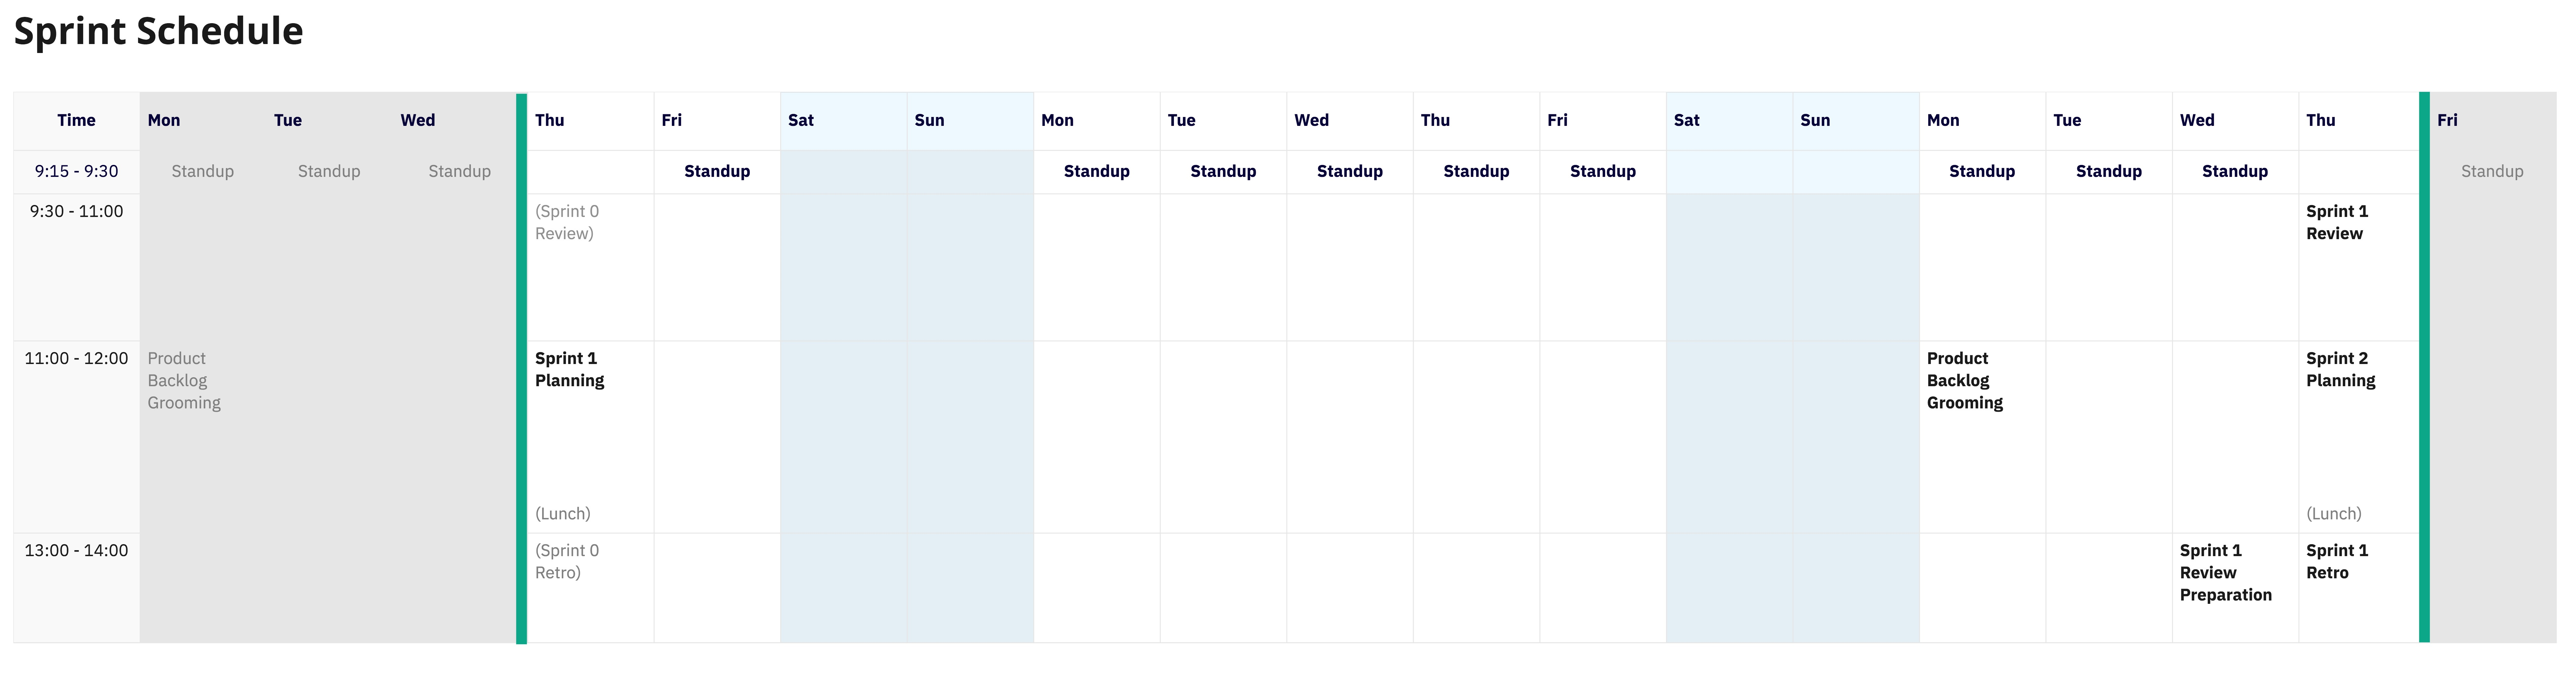
\includegraphics[width=1\textwidth \centering]{sprintschedule.jpeg}
    \caption{Bi-weekly Sprint schedule, shifted Thursday}
    \label{fig:schedule}
\end{figure}
\begin{itemize}
    \item Sprint 1 Planning (Thursday, week 0)
    \item Active Sprint (Thursday, week 0 - week 2) incl. Daily Standups
    \item Sprint 1 Backlog Grooming (Monday, week 2)
    \item Sprint 1 Review (Thursday, week 2)
    \item Sprint 2 Planning  (Thursday, week 2)
    \item Sprint 1 Retro (Thursday, week 2)
\end{itemize}
Each Sprint followed the same Rituals, the execution of which I will describe in our project context further down below (see: \hyperref[sec:rituals]{3.3 Rituals}).
\subsection{Boards}
Our task-management was managed through (task) boards on JIRA.
A board consisted of four columns in the respective order:
\begin{itemize}
    \item To-Do
    \item In Progress
    \item In Review
    \item Done
\end{itemize}
Each new task was assigned to the To-Do column in our "Product Backlog". If we moved a task to the Sprint board, the task was assigned to the respective column of the task state (default: To-Do). 
A task may already have been "In Progress" or "In Review" as part of a previous Sprint and would in such a case be assigned to its previous corresponding state column. 
Our "Product Backlog" existed horizontally separated from the relevant Sprint tasks at the very bottom of the sprint board labelled as “Backlog” in JIRA. 
It followed the same four-column schema as the active Sprint board. Thus, our Sprint board lacked the common one-column “Backlog” known from Kanban (see more: \hyperref[sec:advantages]{4.1 Advantages}). 
All non-started tasks in the Product Backlog were stored in the To-Do column. 
If a task from the backlog should be included into the Sprint, we pulled it from the lower Product Backlog into the top Sprint board.
\subsection{Rituals}
\label{sec:rituals}
\subsubsection{Daily Standups}
Standups happened every weekday for ten scheduled minutes at workday beginning (9:15am). 
We updated each other on the progress, decisions of corporate meetings with our internal stakeholders or blockers we faced the previous day. 
Everyone took their turn, stating at the very least “Good morning! I have nothing new to share, no blockers!”. 
Our Scrum master facilitiated the meeting by screen-sharing the current JIRA Sprint board and navigating to mentioned tickets during the individual standups of the team members. 
\\\linebreak
The talks for tasks requiring collaboration between specific individuals were individually planned after the standup. 
This allowed the standups to be quick informative meetings to stay up-to-date without being caught up in discussions unrelated to your responsibility that day.
\\\linebreak
Especially in the remote setting, the fixed daily standup time was also a great assistance in finding a routine and “start of the day”, which is a factor that should not be underestimated. 
I happily joined the standups even on days I wasn’t working by calendar for that benefit and some colleagues chose to do the same from time to time. 
In my opinion, this is a marker of success for our shared team spirit and execution of the concept of standups.
\subsubsection{Sprint Planning}
At the time when I joined, our product was in a pre-deliver stage to the first customer. 
This implied a lot of cleanups, adjustments, bug fixes and last iterations. 
These tasks were due before release and therefore kept on being relevant if they weren’t finished yet. 
Naturally, the first step of our Sprint Planning was therefore to see which tasks of the last Sprint have been finished and to transfer the unfinished ones into the coming Sprint. 
\\\linebreak
Next were the new open tasks that we decided to tackle this Sprint. 
We selected these on the \hyperref[sec:grooming]{3.3.3 Backlog Grooming} session a few days earlier. 
The relevant part during the Sprint Planning was the estimation of story points for the task. 
We used Planning Poker for that, where everybody gave an estimate of 1 up to 100, following the typical Fibonacci version just with rounded digits towards the end (20, 50, 100). 
As usual, our Scrum Master was non-participative in the progress and facilitated the meeting, with an exception to direct Design decisions since he functioned as our Interaction Designer, too.
\\\linebreak
After a task had been estimated, the task was assigned to a team member. 
We continued this process until all new tasks were estimated and assigned. 
We also sometimes picked up previously estimated tasks to be re-estimated if there was a necessity for it. 
With the estimation and assignment of tasks, we reviewed the distribution of story points throughout the team members. 
If it looked unbalanced, we had to adjust and communicate potential redistributions or constellations of featured tasks in the Sprint. 
Once there was confidence in the manageable distribution of story points, the Sprint was started.

\subsubsection{Backlog Grooming}
\label{sec:grooming}
Our execution of Backlog Grooming was generally done by the book. 
It took at max. an hour, respecting the resources of the development team, and was a get-together to refine and prioritise tasks in the Product Backlog. 
In this meeting, we derived the tickets most important for the next Sprint. 
The meeting was predominantly directed by the Product Owner and Scrum Master.
\subsubsection{Review Preparation}
The Review Preparation happened one day before the finishing Sprint Review. 
This one-hour meeting was fully optional and served as a planned blocker to get together and prepare the final touches or documentation for the presentation of work at the Sprint Review. 
Most of my co-workers frequently used this meeting - I didn’t as it was not aligned with my working schedule.
\subsubsection{Sprint Review}
Our Sprint Review directly preceded the follow-up Sprint Planning for the next two weeks. 
This was the meeting used for presenting for this Sprints progress, so often everyone would share their screen and go through their contributions bit by bit. 
Stakeholders from outside the core team (e.g. Portfolio Manager, cooperating customers) would also join this meeting to get an overview. 
This meeting boosted morale by showcasing the work that had been completed and motivated most of us to attend the Review Preparation or put effort into presenting good work.
\subsubsection{Retrospectives}
The Retrospective (Retro) for the last Sprint followed right after the Planning for the next Sprint. 
For our Retros, we used an online tool to use “Good, Bad, More, Less and Try”. 
Everyone got ten minutes to write their points in the respective column (in a hidden personal space). 
One person at a time would then present their points from Good to Try and further comment on them via voice. 
Following that, we grouped potential similar tickets into one and then each got three votes to distribute on the points we find the most relevant to us. 
From the visibly most upvoted ones, we defined direct action points we can take together, which was the ending activity of our Retrospective (after a warm goodbye).
\section{Reflection}
\subsection{Advantages}
\label{sec:advantages}
In general, the Sprint Plannings worked out great for us. 
The tasks were well estimated and assigned, judging by the history of the success. 
This set a great foundation for exceptionally efficient development phases in our Sprints. 
The Reviews were fun to attend as we encouraged and complemented each other for our work. 
I am convinced that a lot of our meetings went smoothly due to the shared team spirit and respect for another. 
Our Retrospectives were guided by a free room for professional and personal matters, acknowledging that in a remote setting, a week of bad weather can be a fair point for a “Bad” post-it. 
For my team at Porsche, I therefore support the decision to hold the Retrospective for the last Sprint after the Planning for the next Sprint had already happened, as these meetings were a morale booster and kicked-off the energy to tackle the new tasks happily.
\\\linebreak
A word on separating the Product Backlog: I grew to like this approach of a Product Backlog with the same schema as the Sprint board in comparison to a backlog column I was used to from my previous projects at CODE with Kanban for two reasons: 
First, the active board (Sprint board) was now only visualizing the relevant tasks for the upcoming future. 
On top of that, it removed the present long “due list” prepended to the board which one usually has with a backlog column that amplifies the psychological discomfort of “never be done” by constantly seeing the waiting list of tasks in the periphery. 
With a horizontal split into two separate boards, one can remove the backlog (Product) from the relevant task overview (Sprint) while keeping it quickly available if needed.
Additionally, a schemed Product Backlog better visualizes the status of moved-back tickets, which rarely but occasionally happens: A one-column backlog is indiscriminate of the development status of a task, while a schemed backlog can display the current state (e.g. In Progress).
\\\linebreak
I am confident that Scrum was a fitting framework for our project. 
For a period of time, Kanban with a looser development flow would also have worked. 
Especially towards the end of the project when I joined, a lot of the development had to be communicated with the stakeholders and more iterations over concepts had to be made. 
A more time-fixed framework such as Scrum with Sprints allowed us to have clear bi-weekly goals and share results in a predictive timeframe. 
A benefit to the framework was also the experience of the team members with the flow of Scrum. 
Everybody had worked with it for years, knew its advantages and disadvantages, and could therefore avoid traps such as underestimating workloads or having meetings without an agenda.
\subsection{Disadvantages}
Unfortunately, during our rituals, whether it was Planning or Review, we also often got lost in a lot of discussions as a group that only a few individuals would understand (deep technological terms), stretching the meeting and lowering morale. 
As a working student mainly limited to the Frontend development, I found myself in a lot of technical discussions about other development domains I had no experience with. 
Since we had committed to attend to these Rituals as a team, a shift from the agenda implied a measureable impact on all team members. The entire team was effected by a heated argument, although it may have been a discussion reduced to technical decisions within a specific domain.
Most of our ritual meetings took longer than scheduled as discussions around requirements and product roadmap took over the room. 
After a few occasions of these incidents, we identified the action point that a more separate all-hands meeting for reviewing the releasing roadmap and the implied required work had to be held. 
\\\linebreak
The thing I am most inclined to address is the need for improvement in the Rituals agenda on a Thursday. 
The morning started with a 1:30h Review, followed by a 1h Sprint Planning, often directly proceeding into a 1h Retro. 
Even with the planned lunch break inbetween, this was an exhausting “Agile day” due to the amount of discussions, input and simply: Zoom fatigue. 
It took a relaxed evening to recover from that.
\section{Self Evaluation}
I am quite familiar with working in an Agile environment. 
I am used to a Scrum or Kanban setting due to my work as a developing freelancer and my projects at CODE. 
I am comfortable jumping into a project with settings alternating from “the book”, and feel pretty confident picking up frameworks I haven’t worked with yet (e.g. Extreme Programming) due to my education and experience with the Agile fundamentals. 
That being said, I have an intuitive feeling that there are more advanced concepts of Agile or frameworks I haven’t touched on (e.g. XP), and although I'm probably able to comprehend them, I cannot point to or describe them in detail. 
I would therefore assess myself to be at Level 1, albeit on the higher grade boundary of that level. 
\end{document}
